\begin{frame}

Lähtökohtaisesti sähkötyöt ovat kiellettyjä maallikoilta. Lista erikseen sallituista sähkötöistä löytyy esimerkiksi Sähköturvallisuuden edistämiskeskuksen sivuilta
\url{http://www.stek.fi/sahkon_kaytto_kotona/aiotko_tehda_sahkotoita_kotona/fi_FI/sallitut_sahkotyot/}\footnote{Viitattu 14.9.2013}

Listaa ei tarvitse päntätä ulkoa, mutta kokonaiskuva sallituista töistä on hyvä olla mielessä.
\end{frame}


\begin{frame}
\frametitle{Sallitut korjaus- ja asennustyöt}
\begin{itemize}
\item    Yksivaiheisen jatkojohdon korjaus ja teko
\item    Sähkölaitteen rikkoontuneen yksivaiheisen liitäntäjohdon ja pistotulpan vaihto
\item    Valaisimen liitäntäjohdon rikkoontuneen välikytkimen vaihto
\item    Sisustusvalaisimen liittäminen valaisinliitimellä eli ”sokeripalalla”
\item    Kiinteässä asennuksessa valaisinliittimen eli sokeripalan korvaaminen uuden järjestelmän mukaisella valaisinliitinpistorasialla sekä vioittuneen valaisinliitinpistorasian vaihto
\item    Valaisinpistotulpan asennus ja vioittuneen tulpan vaihto
\item    Jännitteettömien pistorasioiden ja kytkimien kansien irrottaminen esim. maalaamisen ja tapetoinnin ajaksi ja rikkoutuneiden kansien vaihto
\item    Suojajännitteisten laitteistojen asentaminen valmistajan tai tavarantoimittajan antamien ohjeiden mukaisesti
\item    Harrastustoimintana tehtävä sähkölaitteiden kokoonpano esim. elektroniikan rakennussarjasta ja tällaisen laitteen korjaaminen
\end{itemize}
\end{frame}



\begin{frame}
\frametitle{Sallitut käyttötoimenpiteet}
\begin{itemize}
\item    Sulakkeen vaihto (tavallisen tulppasulakkeen vaihto tai valonsäätimen sulakkeen vaihto)
\item    Automaattisulakkeen ohjaaminen toiminta-asentoon tai pois päältä
\item    Suojalaitteen toiminta-asennon ohjaaminen
\item    Valaisimen lampun ja sytyttimen vaihto
\item    Jännitteettömyyden toteaminen hyväksytyllä jännitteenkoettimella (koetuskynällä) , kun tehdään jokaiselle sähkönkäyttäjälle sallittuja töitä
\item Vikavirtasuojakytkimen toiminnan testaus
\end{itemize}
\end{frame}

\begin{frame}
\frametitle{Sallittua on myös}
\begin{itemize}
\item    Omakotitalon antennin asentaminen
\item    Sähkölaitteiden mekaanisten osien korjaaminen, esim pesukoneen letkun vaihto, edellyttäen että laitteen kosketussuojaus, vesisuojaus mukaan lukien, ei muutu
\item    Luotettavasti ja kokonaan jännitteettömiksi tehtyjen sähköasennusten purku
\item    Kaapeliojan kaivu ja kaapelin veto maahan. Ennen kaapeliojan peittämistä on sähköalan ammattilaisen todettava, että työ on tehty asianmukaisesti.
\end{itemize}
\end{frame}

\begin{frame}
\frametitle{Laitteiden korjaaminen maallikkona}
Sallittua on
\begin{itemize}
\item Piirikortin vaihto ja lisäys % Ks. Sähkölaitekorjaajan opas s. 5
\item Erilliskoteloidun virtalähteen vaihtaminen.
\item Hybridi- ja sähköajoneuvoissa sellainen huolto- ja korjaustyö, joka on vain pistoliitinkojeen vaihtoa samanlaiseen uuteen, ei vaadi urakointioikeutta (eikä sähkötöiden johtajaa eikä sähköpätevyyttä). Sähköturvallisuudesta on toki huolehdittava ja työntekijöille on annettava SFS 6002:n mukainen sähkötyöturvallisuuskoulutus. % Ks.
\end{itemize}
\end{frame}

\begin{frame}
\frametitle{Sähkölaitteiden suojaustavat}
\begin{itemize}
\item Peruseristys (esim. halpa pöytälamppu).
\item Suojaeristys (parranajokone, porakone)
\item Suojamaadoitus (lämpöpatteri, silitysrauta, sähköhella)
\item Suojajännite (lelut, jouluvalot)
\end{itemize}
\end{frame}

\begin{frame}
\frametitle{Pistotulpat ja kaapelit} % Sähkölaitekorjaajan opas
\begin{itemize}
\item Tavallinen pistotulppa (suojausluokka 0). Ei sovi suojamaadoitettuun pistorasiaan.
\item Suojakosketinpistotulppa (suojausluokka 1).
\item Suojaeristetty pistotulppa (suojausluokka 2).
\end{itemize}

Tavallisen pistotulpan tilalle ei saa vaihtaa suojakosketin- eikä suojaeristettyä pistotulppaa.

Suojaeristetyn pistotulpan tilalle saa vaihtaa suojakosketinpistotulpan. Tällöin suojamaadoitusliitin jätetään kytkemättä.

Verkkojohdon tilalle saa vaihtaa ainoastaan samanlaisen verkkojohdon (mm. johdinpinta-ala, pakkasen-, auringonvalon-, lämmön- ja öljynkestävyys). 

Suojajohdin on jätettävä pidemmäksi kuin muut johtimet, jotta se irtoaa viimeisenä, jos johto revitään väkivalloin irti.

\end{frame}

\begin{frame}
\frametitle{Suojamaadoitus}
\begin{itemize}
\item Käytännössä kaikki metallirunkoiset laitteet ovat suojamaadoitettuja.
\item Jos laitteen sisälle tulee vika, joka meinaa tehdä rungon jännitteiseksi (esimerkiksi leivänpaahtimen vastuslanka katkeaa ja koskee runkoon), vikavirta kulkee rungosta suojamaadoitusliittimen kautta
sähköverkon maahan ja johdonsuojalaite (sulake tai automaattisulake) katkaisee virran.
\item Jos suojamaadoitetun laitteen kytkee tavalliseen pistorasiaan, runko ei ole yhteydessä sähköverkon maahan, ja vian sattuessa runko on jännitteinen $\to$ vaara.
\item Parempi suojaus 
\end{itemize}
\end{frame}

\begin{frame}
\frametitle{Vikavirtasuojakytkin}
\begin{itemize}
\item Pakollinen uudiskohteissa (lähes) kaikissa pistorasioissa.
\item Vikavirtasuojakytkin valvoo vaihe- ja nollajohtimen välistä virtaa. Jos virrat eivät ole yhtä suuret, tämä on merkki viasta (esimerksi ihmisen läpi kulkevasta virrasta) ja vikavirtasuojakytkin katkaisee virran.
\item Vikavirtasuojakytkimiä on saatavilla myös erillisenä pistorasiaan kytkettävänä laitteena. Tällaisen käyttö on suositeltavaa, jos esim. työskentelee ulkona sähkötyökalun kanssa.
\item Vikavirtasuojakytkin suojaa monenlaisilta sähkötapaturmilta. Esimerkiksi kylpyammeeseen putoava hiustenkuivaaja laukaisee välittömästi vikavirtasuojakytkimen.
\end{itemize}
\end{frame}

\begin{frame}
\frametitle{Johtimien merkitseminen}
\begin{itemize}
\item Suojajohdin (PE tai PEN): keltavihreä (ei saa käyttää muuhun!)
\item Nollajohdin (N): sininen
\item Vaihejohtimet (L1, L2, L3): ruskea, musta, harmaa (suositus)
\end{itemize}
Eri aikakausina on käytetty erilaisia värejä, älä luota sokeasti! 

\end{frame}

\begin{frame}
\frametitle{Arkipäivän sähköturvallisuus}
\begin{itemize}
\item Älä sörki avojohtoja.
\item Käytä vikavirtasuojalaitetta, kun käytät sähkötyökaluja.
\item Älä irrota pistotulppaa johdosta vetämällä, vedä aina pistotulpasta.
\item Tarkista aina laite silmämääräisesti. Esimerkiksi murtunut verkkojohto tulee vaihtaa heti. 
\item Varmista jännitteettömyys (koetinkynällä) ennen sähkötöiden tekemistä, ja silloinkin kohtele johtimien metalliosia kuin ne olisivat jännitteisiä.
\item Älä tee sähkötöitä yksin.
\end{itemize}
\begin{block}{Sähkö on turvallista}
Sähkön käyttö on yleisesti ottaen turvallista ja sähkökuolemat harvinaisia. Esimerkiksi kaatumisiin ja putoamisiin kuolee satoja ihmisiä vuodessa ja sähkötapaturmiin alle viisi vuodessa. Tämä ei tarkoita sitä, etteikö kannata olla varovainen.
\end{block}
\tiny \url{http://www.thl.fi/fi_FI/web/pistetapaturmille-fi/tilastot/tilastokatsaukset/kaatumisesta-tai-putoamisesta-aiheutuneet-kuolemat}
\end{frame}

\begin{frame}
\frametitle{Sähkövirran vaikutukset ihmiseen} % D2009
\begin{itemize}
\item Tunto (0,5 mA)
\item Kipu
\item Kouristukset (10 mA)
\item Sydänkammiovärinä (30 mA) ja sydänpysähdys
\item Palovammat ja kemialliset reaktiot (> 100 mA)
\end{itemize}
\end{frame}

\begin{frame}
\frametitle{Ihmiskehon impedanssi}
\begin{itemize}
\item Riippuu kosketuspinta-alasta, henkilöstä, jännitteestä ja taajuudesta.
\item Verkkojännitteellä suuruusluokkaa $1--10\kohm$ % D2009 sivu 45
\end{itemize}
\end{frame}

\begin{frame}
\frametitle{Jännitteet} % SFS 6002
\begin{itemize}
\item Alle 50 Vac tai 120 Vdc = pienoisjännite (ELV)
\item Alle 1000 Vac tai 1500 Vdc = pienjännite (LV)
\item Yli edellä mainituista = suurjännite (HV)
\end{itemize}
\end{frame}

\begin{frame}
\frametitle{Sähkötapaturman ensiapu} % D2009
\begin{itemize}
\item Tee nopea tilannearvio
\item Katkaise virta ja irrota loukkaantunut vaarantamatta itseäsi
\item Tarkista autettavan tila
\item Hälytä apua
\item Anna ensiapua
\end{itemize}
\end{frame}

\begin{frame}
\frametitle{Kuolemaan johtaneet sähkötapaturmat}
Kymmenen vuoden liukuva keskiarvo
\begin{center}
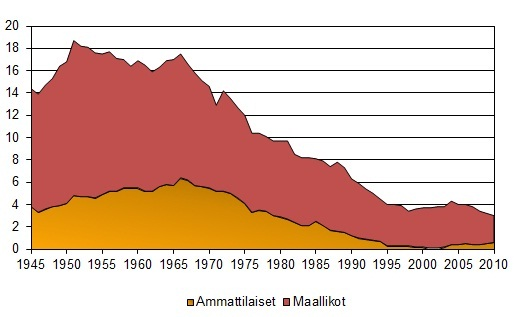
\includegraphics[width=10cm]{sahkoturvallisuus-perusteet_pics/Sahkokuolemat_2010.jpg}
\end{center}

\small \url{http://www.tukes.fi/fi/Rekisterit/sahko-ja-hissit-rekisterit/sahkotapaturmat/kuva-sahkotapaturmat/}
% TODO Mahduta alla olevat kolme riviä siististi kalvolle.
% Kuolemaan johtavien sähkötapaturmien kuvaukset julkistetaan:
% \url{http://www.tukes.fi/fi/Rekisterit/sahko-ja-hissit-rekisterit/sahkotapaturmat/}
% Itsemurhia ei lasketa tapaturmiksi.
\end{frame}

\begin{frame}
\frametitle{Kuolemaan johtaneet sähkötapaturmat 2010}

\begin{itemize}
\item Kytkinlaitosasentaja kuoli latausjännitteeseen valmistellessaan voimajohdon käyttöönottomittausta.
\item Maallikko sai kotipihassaan kuolemaan johtaneen sähköiskun koskettaessaan metallista jatkojohtokelaa. Kela oli tullut jännitteiseksi johtuen siihen tulevan jatkojohdon virheellisestä kytkennästä. 
\item Nuori mies kuoli hypättyään rautatieaseman kävelysillalta alla olevan junan katolle.  
\end{itemize}
\end{frame}

\begin{frame}
\frametitle{Kuolemaan johtaneet sähkötapaturmat 2009}
\begin{itemize}
\item Verkkoyhtiön kolmesta sähköasentajasta koostuva työryhmä oli asentamassa sähköliittymien etäluennan käyttöönottoon liittyvää laitetta 20 kV pylväsmuuntajan kanteen. Työkohde erotettiin muuntajaerottimella (kuormanerotin) ja erottimen avausväli tarkastettiin silmämääräisesti. Muuntajan jännitteettömyyttä ei kuitenkaan varmistettu eikä kohdetta työmaadoitettu ennen töiden aloittamista, minkä seurauksena yksi sähköasentajista sai muuntajaa syöttävästä johdosta tappavan sähköiskun. Johdin oli jännitteinen, koska muuntajan pylväserottimen kolmesta vaiheesta yksi ei ollut auennut.

\item  Nuori mieshenkilö oli jostain syystä kiivennyt aamuyöllä asemalla seisoneen tavarajunan katolle. Hän sai vaunun katolla kuolettavan sähköiskun ja putosi maahan.
\end{itemize}
\end{frame}

\begin{frame}
\frametitle{Kuolemaan johtaneet sähkötapaturmat 2007}
Vuonna 2008 ei sähkökuolemia!
\begin{itemize}
\item Mies menehtyi asunnossaan omatoimisen keittiöremontin yhteydessä. Hän sai sähköasennusten jännitteisestä johdosta sähköiskun, joka meni kädestä käteen. Mies kuoli sairaalassa.
\end{itemize}
\end{frame}


\begin{frame}
\frametitle{Sähköpätevyydet}
Sähkötöiden johtajalla ja käytön johtajalla on oltava riittävä kelpoisuus. Pätevyystodistuksen myöntää Seti Oy. Pätevyyteen vaaditaan
\begin{itemize}
\item Riittävä koulutus
\item Riittävä työkokemus
\item Hyväksytysti suoritettu sähköturvallisuustutkinto
\end{itemize}
\end{frame}

\begin{frame}
\frametitle{Sähköpätevyys 3}
Koulutus ja työkokemus
\begin{itemize}
\item Soveltuva korkeakoulututkinto + 6 kk sähkötyökokemusta.
\item Sähköalan insinööri- tai teknikkotutkinto + 6 kk.
\item Soveltuva (erikois)ammattitutkinto + 6 kk.
\item Soveltuva ammatillinen perustutkinto + 1 v.
\item "Riittävät alan perustiedot" ja 6 vuotta sähkötyökokemusta.
\end{itemize}
\end{frame}

\begin{frame}
\frametitle{Vaatimukset opinnoille}
Kk-tutkinnossa 45 opintopistettä sähköalan opintoja (harjoittelua ja opinnäytetyötä ei lasketa). Opinnoissa on käsiteltävä mm. seuraavat aiheet
\begin{itemize}
\item Teoreettinen sähkötekniikka ja sähkömittaustekniikka
\item Sähköturvallisuussäädökset ja -standardit
\item Sähkötyöturvallisuus
\item Rakennuksen sähköverkko
\item Sähköturvallisuuteen liittyvät tarkastukset
\end{itemize}
Tarkempi lista vaadittavista opinnoista löytyy Henkilö- ja yritysarviointi Seti:n sivuilta \url{http://seti.fi}. Täydentäviä opintoja voi suorittaa myös valmistumisen jälkeen. Oppilaitos antaa pyydettäessä todistuksen, jossa kerrotaan, että opinnot on täydennetty vaatimuksia vastaavaksi.
\end{frame}



\begin{frame}
\frametitle{Lähteitä ja lisälukemista}
Jos sähköturvallisuus kiinnostaa lisää, kannattaa tutustua seuraaviin kirjoihin:

\begin{itemize}
\item {\bf SFS 6002 käytännössä. Sähköinfo Oy. 10. uusittu painos. 2010.} Lyhyt käytännön sähköturvallisuuteen keskittyvä kirja.
\item {\bf D1-2012 Käsikirja rakennusten sähköasennuksista. Sähköinfo Oy. 19. uusittu painos. 2012.} Paksu mutta helppolukuinen ja käytännönläheinen kirja sähköasennuksista ja sähköturvallisuudesta.
\item {\bf Sähkölaitekorjaajan opas. Sähköinfo Oy. 7. uusittu painos. 2010.} 19-sivuinen käytännönläheinen opas sähkölaitteiden korjaamiseen.
\end{itemize}
\end{frame}
